\documentclass{beamer}
\usepackage{packages}
\graphicspath{ {./imgs/}{../imgs/} }

% \usetheme{AnnArbor}
\usetheme{Warsaw}
\usecolortheme{beaver}
\useoutertheme{miniframes}
\setbeamertemplate{headline}{}
\setbeamertemplate{title page}[default][rounded=true]
\setbeamertemplate{frametitle}[default][colsep=0bp,rounded=false,shadow=false]
\setbeamercolor{frametitle}{bg=beaverdarkred,fg=white}
\setbeamercolor{framesubtitle}{bg=darkunq}
\setbeamercolor{title}{fg=beaverdarkred}
\setbeamercolor{subtitle}{fg=beaverdarkred}
\setbeamercolor{author in head/foot}{fg=beaverdarkred,bg=darkgrey}
\setbeamertemplate{footline}
{
    \leavevmode%
    \hbox{%
    \begin{beamercolorbox}[wd=1\paperwidth,ht=2.25ex,dp=1ex,center]{title in head/foot}%
        \usebeamerfont{title in head/foot}\insertshortauthor\insertshorttitle\hspace*{2em}
    \end{beamercolorbox}}%
    \vskip0pt%
}
\setbeamertemplate{itemize item}[triangle]
\setitemize{label=\usebeamerfont*{itemize item}%
  \usebeamercolor[fg]{itemize item}
  \usebeamertemplate{itemize item}}




\title[\texttt{ UNQ -> TIP -> MQL}]{Mumuki Query Learning}
\subtitle{\emph{Un Runner de SQL para el Proyecto Mumuki}}

\titlegraphic{
    
\includegraphics[width=.4\textwidth]{logo-unq}
}

\author[\texttt{Leandro Di Lorenzo ::}]
{
    Leandro~Di~Lorenzo \\
    \textbf{Coordinador:} Ing. Fernando Dodino
    % \vspace{-1em}
}


\institute[TIP - UNQ]
{
   \textsc{
       \small{Tecnicatura en Programación Informática}
   }
}

\date[jul 2017]{8 de Julio, 2017}


\makeatletter
    \newenvironment{withoutheadline}{
        \setbeamertemplate{headline}[default]
        \def\beamer@entrycode{\vspace*{-\headheight}}
    }{}
\makeatother



\begin{document}



%%
%% Carátula
%%
\begin{frame}[plain]
    \titlepage
\end{frame}


%%
%% Problemática
%%
\begin{frame}
    {Problemática y Motivación}
    {\emph{Nuevas formas de enseñar y aprender programación}}

    Al comenzar a programar, una persona se enfrenta a
    desafíos de distinto tipo.

    \vspace{1.5em}

    \begin{columns}[t]
        \column{.5\textwidth}
            El lenguaje de programación:
            \vspace{.5em}
            \begin{itemize}
                \item Paradigma
                \item Sintaxis
                \item Plataforma \\
                      {\footnotesize\emph{Desktop, Web, Mobile, ...}}
                \item Entorno de desarrollo \\
                      {\footnotesize\emph{IDE, Web Server, JVM, ...}}
                \item Compilador / Intérprete
            \end{itemize}

        \column{.5\textwidth}
            Conceptos de programación:
            \vspace{.5em}
            \begin{itemize}
                \item Abstracción
                \item Parametrización
                \item Procedimientos / Funciones
                \item Efecto / Estado
                \item Refactorización
                \item Tipado / Tipos de datos
                \item Legibilidad / Reglas de estilo
            \end{itemize}

    \end{columns}

\end{frame}

\begin{frame}
    {Problemática y Motivación}
    {\emph{El caso Bases de Datos}}

    \begin{itemize}
        \item \emph{Bases de Datos} es una materia de 2do semestre
        \item se viene de cursar \emph{Introducción a la Programación}
        y \emph{Organización de Computadoras}
        \item se cursan en simultáneo con \emph{Programación con Objetos I}
        \item contenidos:
            \begin{itemize}
                \item MER / MR
                \item Normalización
                \item Álgebra Relacional
                \item SQL
            \end{itemize}
    \end{itemize}
\end{frame}

\begin{frame}
    {Problemática y Motivación}
    {\emph{El caso Bases de Datos}}

    \begin{block}{SQL :: Structured Query Language}
        El puente entre la teoría del álgebra relacional y la
        de la programación se logra a partir del \emph{lenguaje SQL},
        el cual permite \textbf{esquematizar y manipular la información}.
    \end{block}

    \vspace{1.5em}

    \begin{columns}[t]
        \column{.5\textwidth}
        Se busca impartir conceptos de:
        \begin{itemize}
            \item Entidad / Atributos
            \item Relación / Cardinalidad
            \item Claves ({\footnotesize\emph{PK, FK}})
            \item Dependencias ({\footnotesize\emph{DFs, DMs}})
        \end{itemize}

        \column{.5\textwidth}
        Y como efecto colateral:
        \begin{itemize}
            \item Motores \\ {\footnotesize\emph{Oracle, Postgres, SQLite, SQL-Server, MySQL, ...}}
            \item Estándares {\footnotesize\emph{ANSI / ISO}}
            \item Portabilidad de datos
        \end{itemize}

    \end{columns}

\end{frame}


%%
%% Proyecto Mumuki
%%
\begin{frame}
    {Propuesta}
    {\emph{Integrar SQL como parte del Proyecto Mumuki}}

    \begin{figure}[h]
        
\includegraphics[width=1\textwidth]{proyecto-mumuki}
    \end{figure}
\end{frame}


%%
%% Un poco de data...
%%
\begin{frame}
    {Mumuki}
    {\emph{Un poco de data...}}
    \begin{itemize}%[<+->]
        \item Mumuki es una plataforma educativa para la enseñanza de programación, y es \textit{Open Source}.
        \item Se puede utilizar de forma autodidacta o como aula virtual con seguimiento.
        \item Es desarrollada y mantenida por estudiantes y docentes de varias universidades públicas, incluída la UNQ.
        \item Está siendo utilizada en diferentes entidades educativas del país.
        \item Tiene un enfoque didáctico con fuerte incapié en los conceptos por sobre las tecnologías.
    \end{itemize}
\end{frame}


%%
%% Mumuki :: Ejercicios
%%
\begin{frame}
    {Mumuki Tour}
    {\emph{Interfaz de ejercicios}}
    \begin{figure}[h]
        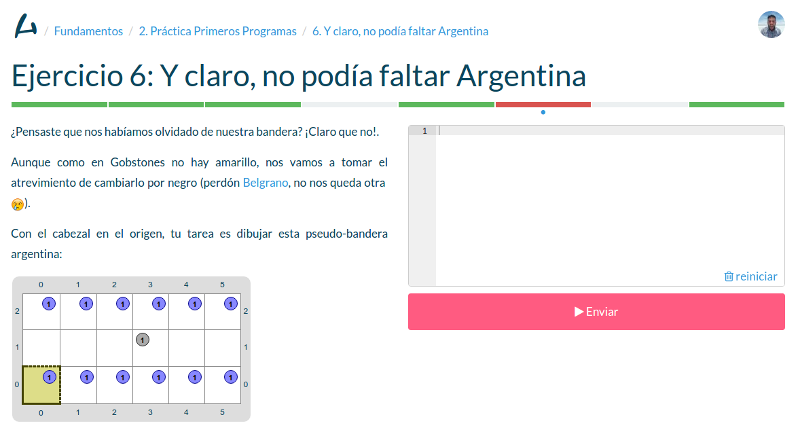
\includegraphics[width=1\textwidth]{gobstones-exercise}
    \end{figure}
\end{frame}

%%
%% Mumuki :: Corrección Automatizada
%%
\begin{frame}
    {Mumuki Tour}
    {\emph{Muestra de errores}}

    \begin{figure}[h]
        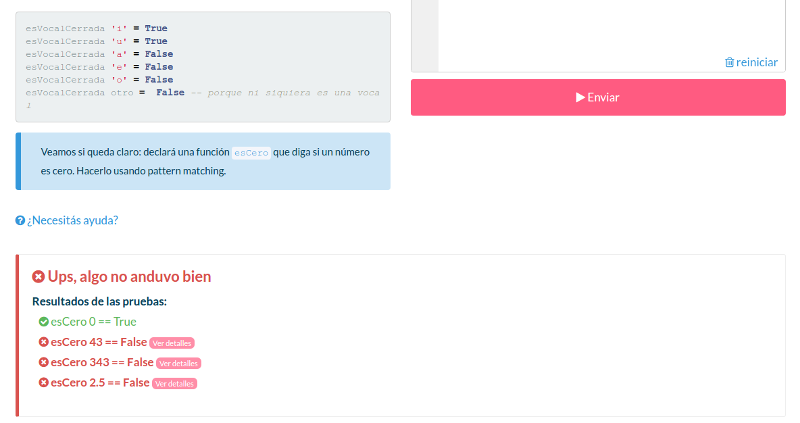
\includegraphics[width=1\textwidth]{haskell-ups}
    \end{figure}
\end{frame}

%%
%% Mumuki :: Seguimiento
%%
\begin{frame}
    {Mumuki Tour}
    {\emph{Aula virtual}}

    \begin{figure}[h]
        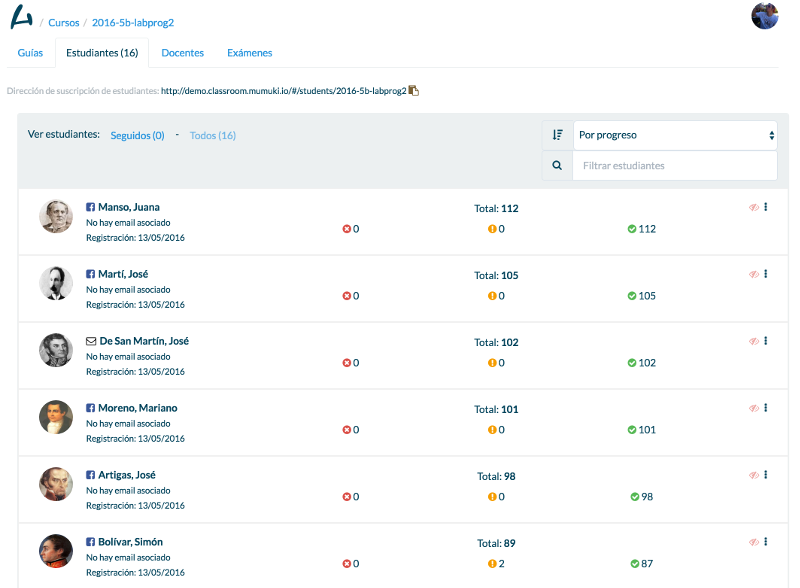
\includegraphics[width=1\textwidth]{classroom-students}
    \end{figure}
\end{frame}




%%
%% Mumuki :: Versionado
%%
\begin{frame}
    {Mumuki Tour}
    {\emph{Seguimiento personalizado}}

    \begin{figure}[h]
        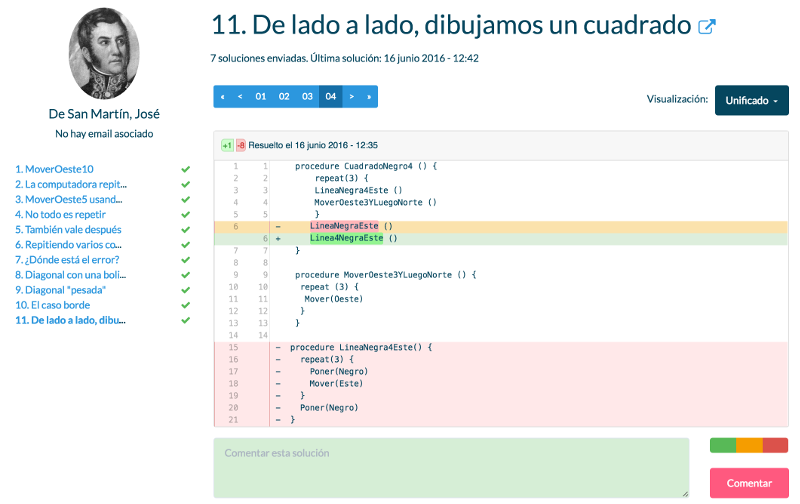
\includegraphics[width=1\textwidth]{classroom-student-detail}
    \end{figure}
\end{frame}

\begin{frame}
    {Plataforma Mumuki}
    {\emph{Componentes}}

    La \textbf{Plataforma Mumuki} se puede entender desde estos componentes:

    \vspace{1.5em}

    \begin{description}
        \item[Laboratory] entorno web en donde los estudiantes resuelven ejercicios
        y reciben \emph{feedback}
        \item[Classroom] herramienta para que el docente pueda generar seguimiento de sus alumnos
        \item[Bibliotheca] repositorio de guías y ejercicios
        \item[Runners] componentes que se encargan de ejecutar y verificar los programas enviados por los alumnos
    \end{description}


\end{frame}


\begin{frame}
    {Plataforma Mumuki}
    {\emph{Los Runners}}

    \begin{itemize}
        \item Un \emph{Runner} se encarga de ejecutar una tecnología en particular
        \item Existen \emph{Runners} de todo tipo de tecnología comercial \\
        {\footnotesize\emph{Java, Ruby, Python, Javascript, C++, Haskell, Prolog, ...}}
        \item Y también \emph{Runners} de tecnologías educativas \\
        {\footnotesize\emph{Gobstones, Wollok, QSIM, ...}}
        \item Cada ejercicio se asocia con el \emph{Runner} de la tecnología necesaria
        \item Cuando un alumno envía la solución de un ejercicio, Mumukit
        genera una petición al \emph{Runner} asociado
        \item El \emph{Runner} compila o interpreta el ejercicio, lo ejecuta y retorna
        los resultados luego de todas las verificaciones realizadas
    \end{itemize}
\end{frame}

\begin{frame}
    {Plataforma Mumuki}
    {\emph{Los Runners}}

    \vspace{-.9em}
    \begin{figure}[h]
        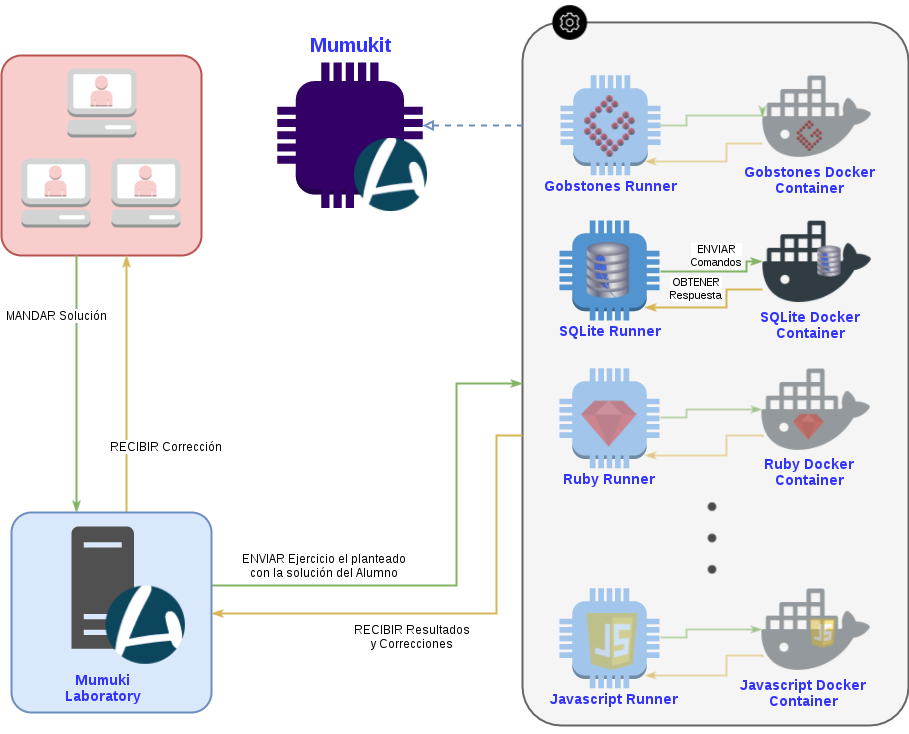
\includegraphics[height=.8\textheight]{MQL-Arquitectura}
    \end{figure}
\end{frame}


\begin{frame}
    {Un Runner para SQL}
    {\emph{Stack Tecnológico}}

    \begin{itemize}
        \item Los \emph{Runners} de Mumuki deben estar programados
        como una gema de \emph{ruby} utilizando el framework \emph{Mumukit}
        \item \emph{Mumukit} se encarga de establecer la interacción con
        la plataforma y delegar el trabajo puntual al \emph{Runner} correspondiente
        \item Cada \emph{Runner} debe tener asociado un \emph{Docker Container}
        \item \emph{Docker} plantea una forma de virtualización en donde
        se pueden crear y destruir \emph{VMs} de forma muy veloz y a bajo costo
        \item La ventaja de utilizar \emph{Docker} es la posibilidad
        de ejecutar cada ejercicio de cada alumno en un ambiente
        aislado y limpio.
    \end{itemize}
\end{frame}

\begin{frame}
    {Runner SQLite}
    {\emph{Stack \& Flow}}

    \begin{figure}[h]
        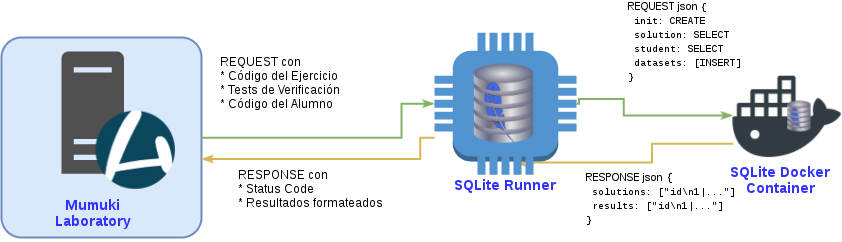
\includegraphics[width=1\textwidth ]{sqlite-flow}
    \end{figure}
\end{frame}

\begin{frame}
    {Runner SQLite}
    {\emph{Stack \& Flow}}

    \begin{itemize}
        \item El \emph{Runner SQLite} adapta el contenido a un formato
        cómodo de manipular por el \emph{worker} (docker container)
        \item El \emph{container} es una VM con: {\footnotesize linux alpine, sqlite3 y python 2.7}
        \item Se inicia un \emph{container} fresco que recibe el ejercicio
        a ejecutar en formato \emph{json}
        \item A través de un script en \emph{python} se crea la base, se inicializa
        el ejercicio y se ejecutan las soluciones del alumno y del docente
        para cada set de datos
        \item Los resultados se retornan en formato \emph{json} junto al
        \emph{exit code}
    \end{itemize}

\end{frame}


\begin{frame}[fragile]
    {Runner SQLite}
    {\emph{Ejemplo I}}
    Ejemplo de un ejercicio de tipo \texttt{SELECT} con solución vía \textit{Query}

\begin{columns}[t]
    \column{.5\textwidth}
    \begin{listing}[H]
        \caption{Extra (Docente, SQL)}
        \begin{minted}[fontsize=\scriptsize]{sql}
    CREATE TABLE motores (
        id integer primary key,
        nombre varchar(200) NOT NULL
    );
        \end{minted}
    \end{listing}

    \begin{listing}[H]
        \caption{Content (Alumno, SQL)}
        \begin{minted}[fontsize=\scriptsize]{sql}
        SELECT id, nombre
        FROM motores;
        \end{minted}
    \end{listing}

    \column{.5\textwidth}
    \begin{listing}[H]
        \caption{Test (Docente, YAML)}
        \begin{minted}[fontsize=\tiny]{yaml}
solution_type: query
solution_query: select * from motores;
examples:
  - data: |
      INSERT INTO motores values ('MySQL');
      INSERT INTO motores values ('PostgreSQL');
      INSERT INTO motores values ('Oracle');
      INSERT INTO motores values ('SQL Server');
      INSERT INTO motores values ('SQLite');
        \end{minted}
    \end{listing}

\end{columns}

\end{frame}

\begin{frame}[fragile]
    {Runner SQLite}
    {\emph{Ejemplo II}}
    Ejemplo de un ejercicio con solución vía \textit{Datasets}

\begin{columns}[t]
    \column{.5\textwidth}
    \begin{listing}[H]
        \caption{Extra (Doc)}
        \begin{minted}[fontsize=\scriptsize]{sql}
CREATE TABLE motores (
    id integer primary key,
    nombre varchar(200) NOT NULL
);
        \end{minted}
    \end{listing}

    \begin{listing}[H]
        \caption{Content (Alu)}
        \begin{minted}[fontsize=\scriptsize]{sql}
        SELECT id, nombre
        FROM motores;
        \end{minted}
    \end{listing}

    \column{.5\textwidth}
    \begin{listing}[H]
        \caption{Test (Doc)}
        \begin{minted}[fontsize=\tiny]{yaml}
solution_type: "datasets"
examples:
  - data: |
      INSERT INTO motores values ('MySQL');
      INSERT INTO motores values ('PostgreSQL');
      INSERT INTO motores values ('Oracle');
      INSERT INTO motores values ('SQL Server');
      INSERT INTO motores values ('SQLite');
    solution_dataset: |
      id|color
      1|MySQL
      2|PostgreSQL
      3|Oracle
      4|SQL Server
      4|SQLite
        \end{minted}
    \end{listing}

\end{columns}

\end{frame}

\begin{frame}[fragile]
    {Runner SQLite}
    {\emph{Ejemplo III}}
    Ejemplo de un ejercicio de tipo \texttt{CREATE} con solución vía \textit{Datasets}

\begin{columns}[t]
    \column{.5\textwidth}
    \begin{listing}[H]
        \caption{Extra (Docente, SQL)}
        \begin{minted}[fontsize=\scriptsize]{sql}
    -- NONE
        \end{minted}
    \end{listing}

    \begin{listing}[H]
        \caption{Content (Alumno, SQL)}
        \begin{minted}[fontsize=\tiny]{sql}
    CREATE TABLE motores (
        id integer primary key,
        nombre varchar(200) NOT NULL
    );

    INSERT INTO motores values ('MySQL');
    INSERT INTO motores values ('PostgreSQL');
    INSERT INTO motores values ('Oracle');
    INSERT INTO motores values ('SQL Server');
    INSERT INTO motores values ('SQLite');

    SELECT * FROM motores;
        \end{minted}
    \end{listing}

    \column{.5\textwidth}
    \begin{listing}[H]
        \caption{Test (Docente, YAML)}
        \begin{minted}[fontsize=\tiny]{yaml}
solution_type: datasets
examples:
  - data: -- none
    solution_dataset: |
      id|color
      1|MySQL
      2|PostgreSQL
      3|Oracle
      4|SQL Server
      4|SQLite
        \end{minted}
    \end{listing}

\end{columns}

\end{frame}


\begin{frame}

    \begin{center}
        \LARGE{DEMO}

        \begin{figure}[h]
            
\includegraphics[width=.6\textwidth]{demo}
        \end{figure}
    \end{center}

\end{frame}


%%
%% Mumuki Query Learning :: Objetivos
%%
\begin{frame}
    {MQL}
    {\emph{Objetivos}}

    \begin{itemize}
        \item Brindar herramientas de \textit{Bases de Datos} para

        \begin{itemize}
            \item Mejorar la didáctica de SQL
            \item Facilitar el seguimiento del alumno
            \item Contar con mejores elementos de evaluación
        \end{itemize}

        \item Permitirle al alumno

        \begin{itemize}
            \item Revisar su progreso
            \item Recibir \emph{feedback online}
            \item Interacturar como comunidad sobre la temática
        \end{itemize}

        \item Hacer un aporte al \textit{Proyecto Mumuki} como \\ comunidad \emph{Open Source}
    \end{itemize}

\end{frame}


%%
%% Consecuencias Deseadas
%%
\begin{frame}
    {MQL}
    {\emph{A Futuro...}}

    Dejar abierta la posibilidad de incorporar tecnología para la enseñanza de:

    \begin{itemize}
        \item Álgebra Relacional

        \item BBDD orientadas a

        \begin{itemize}
            \item Documentos {\footnotesize (\emph{mongoDB})}
            \item Grafos {\footnotesize (\emph{neo4j})}
        \end{itemize}

    \end{itemize}

\end{frame}





%%
%% Algunos Links
%%
\begin{frame}
    {MQL}
    {\emph{Referencias}}

    \begin{thebibliography}{10}
      \setbeamertemplate{bibliography item}[book]
      \bibitem{sadosky}
        Una propuesta para refundar la enseñanza de la computación en las escuelas Argentinas
        \newblock {\em Fundación Sadosky}
        \newblock {\footnotesize \url{http://www.fundacionsadosky.org.ar/wp-content/uploads/2014/06/cc-2016.pdf}}

      \setbeamertemplate{bibliography item}[book]
      \bibitem{gobstones}
        Las bases conceptuales de la Programación: Una nueva forma de aprender a programar
        \newblock {\em Pablo E. Martínez López}
        \newblock {\footnotesize \url{http://www.gobstones.org/bibliografia/Libros/BasesConceptualesProg.pdf}}

      \setbeamertemplate{bibliography item}[article]
      \bibitem{mumuki}
        Mumuki, una plataforma libre para aprender a programar
        \newblock {\em Federico Aloi, Franco Bulgarelli, Lucas Spigariol}
        \newblock {\footnotesize \url{https://www.academia.edu/25374997/Mumuki\_una\_plataforma\_libre\_para\_aprender\_a\_programar}}
      \end{thebibliography}
\end{frame}

%%
%% Algunos Links
%%
\begin{frame}
    {MQL}
    {\emph{Links}}

    \setbeamercolor{bibliography entry location}{fg=black}
    \setbeamercolor{bibliography entry note}{fg=black}

    \begin{thebibliography}{10}
      \setbeamertemplate{bibliography item}[online]
      \bibitem{lmumuki}
        Proyecto Mumuki
        \newblock {\footnotesize \url{http://www.mumuki.org/}}

      \setbeamertemplate{bibliography item}[online]
      \bibitem{runner}
        Runner SQLite
        \newblock {\footnotesize \url{https://github.com/leandrojdl/mumuki-sqlite-runner}}
        \newblock {\footnotesize \url{https://github.com/mumuki/mumuki-sqlite-runner}}

      \setbeamertemplate{bibliography item}[online]
      \bibitem{mumuki}
        Stack Tecnológico
        \newblock {\footnotesize \url{https://www.ruby-lang.org/}}
        \newblock {\footnotesize \url{https://www.sqlite.org/}}
        \newblock {\footnotesize \url{https://www.docker.com/}}
        \newblock {\footnotesize \url{https://www.python.org/}}

      \end{thebibliography}
\end{frame}



%%
%% Gracias :: Preguntas
%%
\begin{frame}
    \begin{center}
        \begin{figure}[h]
            
\includegraphics[scale=.7]{questions}
        \end{figure}
        \vspace{1em}
        \Large{¿Preguntas, ideas, comentarios?}
    \end{center}
\end{frame}

\begin{frame}
    \begin{center}

        \vspace{4em}
        \huge{Muchas Gracias}

        \begin{figure}[h]
            
\includegraphics[scale=.1]{12cactus}
        \end{figure}

    \end{center}
\end{frame}

\end{document}
